\chapter{Input and Output}

\begin{exercise}
Modify the program you wrote in Exercise~\ref{ex:age} to prompt the user for their age in years.
\end{exercise}

\begin{exercise}
\label{ex:dewpoint2}
Modify the program you wrote in Exercise~\ref{ex:dewpoint} to prompt the user for the air temperature and relative humidity. Use \java{printf} to display the dew point with one digit to the right of the decimal point.
\end{exercise}

\begin{exercise}
Modify the program you wrote in Exercise~\ref{ex:heatindex} to prompt the user for the air temperature and relative humidity. Use \java{printf} to display the heat index temperature with one digit to the right of the decimal point.
\end{exercise}

\begin{exercise}
\label{ex:electricvehicle1}
In the United States, the ``fuel efficiency'' of an electric vehicle is measured in miles per kilowatt-hour (kWh). In Canada and Europe, it is measured in kWh per 100km. Write a program that prompts the user for efficiency in miles/kWh . The program will then calculate and display the equivalent efficiency in terms of kwH per/100km. One kilometer equals 0.621371 mile (or, if you prefer, one mile equals 1.609341 km). Here is what the output might look like:

\begin{stdout}
Enter miles per kilowatt-hour: 4.5
That is equivalent to 13.81 kWh/100km.
\end{stdout}

\end{exercise}

\begin{exercise}
\label{ex:electricvehicle2}
In Canada and Europe, the ``fuel efficiency'' of an electric vehicle is measured in kWh per 100km. In the United States, it is measured in miles per kilowatt-hour (kWh).  Write a program that prompts the user for electric vehicle efficiency in kwH/100km and calculates the equivalent in terms of miles/kWh.  One kilometer equals 0.621371 mile (or, if you prefer, one mile equals 1.609341 km). Here is what the output might look like.

\begin{stdout}
Enter kilowatt-hours per 100km: 13.5
That is equivalent to 4.62 miles/kWh.
\end{stdout}
\end{exercise}


\begin{exercise} 
\label{ex:purchase}

The goal of this exercise is to calculate the price of an order given an item's price, the quantity purchased, and the sales tax.
When it's finished, it should work like this:

\begin{stdout}
Please enter the unit price of the item $2.45
Enter the number you wish to purchase: 5

Subtotal:     $12.25
Tax at 7.50%:   0.92
Total:        $13.17
\end{stdout}

Note: the dollar sign in the first line is part of the prompt; the user does not enter the dollar sign.
Use \java{printf} to display exactly two digits to the right of the decimal point.

\end{exercise}


\begin{exercise}
\label{ex.degrees}
Because the \java{Scanner} class views input as a stream of characters, you can ask users for multiple inputs with a single prompt. For example, instead of asking the user for the width and height of a rectangle as two inputs in this code fragment:

\begin{code}
// ask for length in cm
System.out.print("Enter width of rectangle in cm: ");
double width = input.nextDouble();
        
System.out.print("Enter height of rectangle in cm: ");
double height = input.nextDouble();
\end{code}

Which looks like this when the program runs:

\begin{stdout}
Enter width of rectangle in cm: 5.3
Enter height of rectangle in cm: 2.6
\end{stdout}

You could use one prompt:

\begin{code}
System.out.println("Enter width and height of rectangle");
System.out.print("in cm separated by spaces: ");
double width = input.nextDouble();
double height = input.nextDouble();
\end{code}

Which looks like this when the program runs:

\begin{stdout}
Enter width and height of rectangle
in cm separated by spaces: 5.3 2.6
\end{stdout}

In this exercise, you will prompt the user to enter an angle as degrees, minutes, and seconds and convert it to decimal degrees. Here is what the output might look like:

\begin{stdout}
Enter degrees, minutes, and seconds
separated by spaces: 25 15 30
That is 25.2583 degrees (decimal).
\end{stdout}

You may use either one prompt, as shown here, or three separate prompts.

\end{exercise}

\begin{exercise}
\label{brakingDistance}

This is another exercise that uses input and arithmetic operators to calculate the stopping distance for a vehicle. Write a program that prompts the user to enter:

\begin{itemize}

\item The initial velocity in kilometers per hour (\java{double}). A velocity of 60 miles per hour works out to about 97 kilometers per hour.
\item The reaction time in seconds (\java{double}). For most people, the reaction time is about 1.5 seconds.
\item The coefficient of friction for the tires (\java{double}). This is a dimensionless number, normally about 0.7.

\end{itemize}

Calculate and display the stopping distance using this formula:
$d = v \cdot t + {v^2 \over {2 \mu g}}$
where $t$ is the reaction time, $v$ is the initial velocity in {\bf meters per second}, $\mu$ is the coefficient of friction between the tires and the roadway, and $g$ is the acceleration of gravity in meters per second squared. Make $g$ a constant with the value 9.80665.

Notice that, since you are asking for the velocity in kilometers per hour, you must convert it to meters per second. Define constants \java{METERS_PER_KM} (1000) and \java{SECONDS_PER_HOUR} (3600) to use in this calculation.

Here is an example of what the program should look like:

\begin{stdout}
Stopping Distance Calculator
Enter velocity of vehicle in kilometers per hour: 97
Enter reaction time in seconds (normal is 1.5): 1.1
Enter coefficient of friction (from 0.1 to 1.0; normal 0.7): 0.5

Stopping distance is 103 meters.
\end{stdout}

In this program, it is better to use three separate prompts for the input because, unlike Exercise~\ref{ex.degrees}, the entries are not closely related to each other.
 
\end{exercise}

\begin{exercise}
The goal of this exercise is to show the need for planning a program. The calculations themselves are not sophisticated, but figuring out {\em what} those calculations are requires some thinking.

Consider a staircase as shown in Figure~\ref{fig.staircase}.

\begin{figure}[!h]
\begin{center}
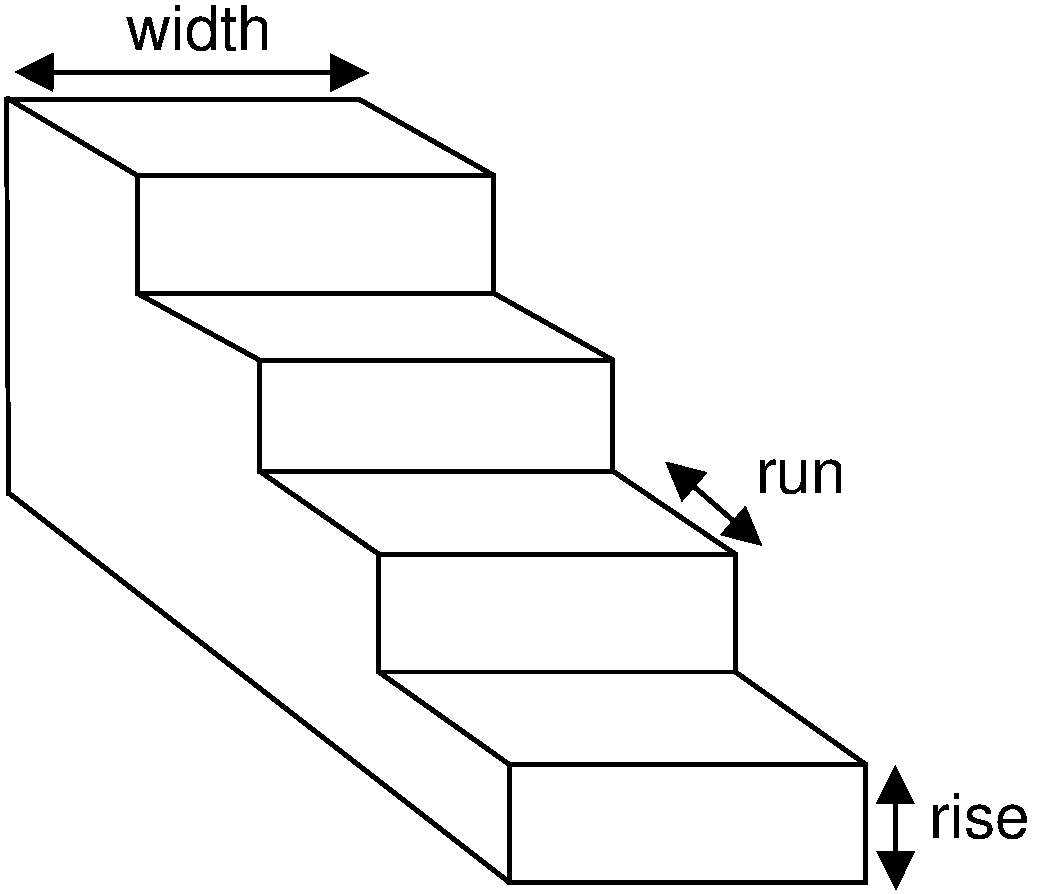
\includegraphics[scale=0.3]{figs/ch03/staircase.pdf}
\caption{A staircase showing the width, the {\em rise} (height), and the {\em run} (depth) of a step.}
\label{fig.staircase}
\end{center}
\end{figure}

Your job is to write a program that prompts the user for the number of steps in the staircase. It will then prompt for and read the width, rise, and run of a step in centimeters. The program will then calculate the number of cubic centimeters of concrete necessary to build the staircase. Round the number of cubic centimeters by adding 0.5 to the calculated volume and then casting that result to an integer.  In general,

\begin{code}
double x;
int xRounded = (int) (x + 0.5);
\end{code}

Calculate by hand what the result of this code would be when \java{x} is 3.4 and again when \java{x} is 3.6 to understand why this code works.

{\em Hints:} How many ``blocks'' the size of the bottom step do you need to build the staircase? Drawing a diagram {\em really} helps. To find the sum of the numbers 1 through n, use this formula: 

\begin{equation*}
sum = {{n(n+1)}\over 2}
\end{equation*}

Here is what program output might look like:

\begin{stdout}
Staircase Volume Calculator
How many steps in the staircase? 5
Enter step width in cm: 45
Enter run of the step in cm: 20
Enter rise of the step in cm: 7.5
Total volume is 101250 cubic centimeters.
\end{stdout}
\end{exercise}


